\documentclass[a4paper,14pt]{extarticle}

\usepackage[utf8x]{inputenc}
\usepackage[T1,T2A]{fontenc}
\usepackage[russian]{babel}
\usepackage{hyperref}
\usepackage{indentfirst}
\usepackage{here}
\usepackage{array}
\usepackage{graphicx}
\usepackage{caption}
\usepackage{subcaption}
\usepackage{chngcntr}
\usepackage{amsmath}
\usepackage{amssymb}
\usepackage{amsthm}
\usepackage{pgfplots}
\usepackage{pgfplotstable}
\usepackage[left=2cm,right=2cm,top=2cm,bottom=2cm,bindingoffset=0cm]{geometry}
\usepackage{multicol}
\usepackage{askmaps}
\usepackage{titlesec}
\usepackage{listings}
\usepackage{color}
\usepackage{enumerate}
\usepackage{hhline}
\usepackage{enumitem}
\usepackage{courier}
\usepackage{wrapfig}
\usetikzlibrary{arrows,automata}

\setitemize{itemsep=0em}
\setenumerate{itemsep=0em}

\theoremstyle{definition}

\pgfkeys{/pgf/number format/.cd,1000 sep={\,}}

\definecolor{green}{rgb}{0,0.6,0}
\definecolor{gray}{rgb}{0.5,0.5,0.5}
\definecolor{purple}{rgb}{0.58,0,0.82}

\lstset{
	language=python,
	backgroundcolor=\color{white},   
	commentstyle=\color{green},
	keywordstyle=\color{blue},
	numberstyle=\tiny\color{gray},
	stringstyle=\color{purple},
	basicstyle=\footnotesize\ttfamily,
	breakatwhitespace=false,
	breaklines=true,
	captionpos=b,
	keepspaces=true,
	numbers=left,
	numbersep=5pt,
	showspaces=false,
	showstringspaces=false,
	showtabs=false,
	tabsize=2,
	frame=single,
	inputpath={../code/}
}

\renewcommand{\le}{\ensuremath{\leqslant}}
\renewcommand{\leq}{\ensuremath{\leqslant}}
\renewcommand{\ge}{\ensuremath{\geqslant}}
\renewcommand{\geq}{\ensuremath{\geqslant}}
\renewcommand{\epsilon}{\ensuremath{\varepsilon}}
\renewcommand{\phi}{\ensuremath{\varphi}}
\renewcommand{\thefigure}{\arabic{figure}} 	
\newcommand{\norm}[1]{\left\lVert#1\right\rVert}
\newcommand*\sfrac[2]{{}^{#1}\!/_{#2}}

%\titleformat*{\section}{\large\bfseries} 
\titleformat*{\subsection}{\normalsize\bfseries} 
\titleformat*{\subsubsection}{\normalsize\bfseries} 
\titleformat*{\paragraph}{\normalsize\bfseries} 
\titleformat*{\subparagraph}{\normalsize\bfseries} 

\counterwithin{figure}{section}
\counterwithin{equation}{section}
\counterwithin{table}{section}
\newcommand{\sign}[1][5cm]{\makebox[#1]{\hrulefill}}
\graphicspath{{../pics/}}
\captionsetup{justification=centering,margin=1cm}
\setlength\parindent{5ex}
\def\arraystretch{1.3}
\def\tabcolsep{12pt}
%\titlelabel{\thetitle.\quad}

\DeclareMathOperator*{\argmin}{argmin}
\DeclareMathOperator*{\argmax}{argmax}

\begin{document}

\begin{titlepage}
\begin{center}
	\textbf{Санкт-Петербургский Политехнический Университет \\Петра Великого}\\[0.3cm]
	\small Институт компьютерных наук и технологий \\[0.3cm]
	\small Кафедра компьютерных систем и программных технологий\\[4cm]
	
	\textbf{ОТЧЕТ}\\ \textbf{по расчетному заданию}\\[0.5cm]
	\textbf{<<Построение моделей>>}\\[0.1cm]
	\textbf{Системный анализ и принятие решений}\\[8.0cm]
\end{center}

\begin{flushright}
	\begin{minipage}{0.4\textwidth}
		\begin{flushleft}
			\small \textbf{Работу выполнил студент}\\[3mm]
			\small группа 33501/4 \hspace*{6mm} Дьячков В.В.\\[5mm]
			
			\small \textbf{Преподаватель}\\[5mm]
		 	\small \sign[3cm] \hspace*{5mm} Сабонис С.С.\\[0.5cm]
		\end{flushleft}
	\end{minipage}
\end{flushright}

\vfill

\begin{center}
	\small Санкт-Петербург\\
	\small \the\year
\end{center}
\end{titlepage}

\addtocounter{page}{1}

\tableofcontents
\listoftables
\listoffigures
\newpage

\section{Техническое задание}

\begin{itemize}
	\item Задача сетевого планирования, метод динамического
	программирования. На основе графа, приведенного на рис. \ref{fig:graph}:
	\begin{enumerate}
		\item написать матрицу смежности;
		\item определить наиболее ранние моменты наступления событий;
		\item определить наиболее поздние моменты наступления событий;
		\item определить резервы времени, написать матрицу резервов;
		\item найти критический путь (пути);
		\item определить минимально возможное время выполнения всего комплекса работ.
	\end{enumerate}
	\item Для $n = 1$ определить время выполнения всего комплекса работ;
	\item Для $n = 3$ найти распределение работ по ресурсам, рассмотреть 4 критерия выбора работ для выполнения, указанные ниже; для каждого критерия привести решение задачи по шагам, построить график, найти общее время работы, найти времена простоя каждого ресурса:
	\begin{enumerate}
		\item работа наименьшей длительности;
		\item работа наибольшей длительности;
		\item работа с наименьшим резервом;
		\item работа с наибольшим резервом. 
	\end{enumerate}
\end{itemize}

\vspace{-0.5cm}
\section{Исходные данные}

\begin{figure}[H]
\begin{center}
	\begin{tikzpicture}[->,>=stealth',shorten >=1pt,auto,node distance=2.8cm,
	                    semithick, inner sep=5pt]
	  \tikzstyle{every state}=[fill=white,draw=black,text=black]
	
	  \node[initial, state]	(1) 					{$1$};
	  \node[state] 			(2) [right of=1] 		{$2$};
	  \node[state] 			(3) [above right of=2] 	{$3$};
	  \node[state] 			(4) [below right of=2] 	{$4$};
	  \node[state] 			(5) [below right of=3] 	{$5$};
	  \node[state] 			(6) [below right of=5] 	{$6$};
	  \node[state] 			(7) [below right of=4] 	{$7$};
	  \node[state] 			(8) [above right of=6] 	{$8$};
	  \node[state] 			(9) [right of=8] 		{$9$};
	
	  \path (1)	edge 				node 		{6} (2)
	  			edge [bend left] 	node 		{7} (3)
	  			edge [bend right] 	node [swap] {4} (4)
	  		(2) edge 				node 		{6} (3)
	  			edge 				node 		{4} (4)
	  		(3) edge 				node 		{5} (5)
	  			edge [bend left] 	node 		{5} (8)
	  		(4) edge 				node 		{6} (5)
	  			edge 				node [swap] {4} (6)
	  			edge [bend right] 	node [swap] {6} (7)
	  		(5) edge 				node		{4} (6)
	  			edge 				node 		{3} (8)
	  		(6) edge 				node 		{5} (8)
	  		(7) edge [bend right] 	node [swap] {7} (8)
	  		(8) edge 				node 		{4} (9);
	\end{tikzpicture}
	\caption{Исходный граф (вариант 32)}
	\label{fig:graph}
\end{center}
\end{figure}

\section{Задача сетевого планирования}

\subsection{Матрица смежности}

\begin{table}[H]
	\centering
	\def\tabcolsep{12pt}
	\caption{Матрица смежности}
	\label{tab:1}
	\begin{tabular}{|c|c|c|c|c|c|c|c|c|c|}
		\hline
		\bf{№} & \bf{1} & \bf{2} & \bf{3} & \bf{4} & \bf{5} & \bf{6} & \bf{7} & \bf{8} & \bf{9} \\
		\hline
		\bf{1} & - & 6 & 7 & 4 & - & - & - & - & - \\ 
		\hline
		\bf{2} & - & - & 6 & 4 & - & - & - & - & - \\ 
		\hline
		\bf{3} & - & - & - & - & 5 & - & - & 5 & - \\ 
		\hline
		\bf{4} & - & - & - & - & 6 & 4 & 6 & - & - \\ 
		\hline
		\bf{5} & - & - & - & - & - & 4 & - & 3 & - \\ 
		\hline
		\bf{6} & - & - & - & - & - & - & - & 5 & - \\ 
		\hline
		\bf{7} & - & - & - & - & - & - & - & 7 & - \\ 
		\hline
		\bf{8} & - & - & - & - & - & - & - & - & 4 \\ 
		\hline
		\bf{9} & - & - & - & - & - & - & - & - & - \\ 
		\hline
	\end{tabular}
\end{table}

\subsection{Наиболее ранние и поздние моменты наступления событий}

На рис. \ref{fig:events} приведен исходный граф с обозначенными в нем наиболее ранними $t_i'$ и наиболее поздними моментами $t_i''$ наступления событий, указанными внутри событий как $\sfrac{t_i'}{t_i''}$. На ребрах графа после веса в скобках указан резерв выполнения работы $r_{ij}$.

\begin{figure}[H]
	\begin{center}
		\begin{tikzpicture}[->,>=stealth',shorten >=1pt,auto,node distance=2.8cm,
		semithick, inner sep=5pt]
		\tikzstyle{every state}=[fill=white,draw=black,text=black]
		
		\node[initial, state]	(1) 					{$1 \atop \sfrac{0}{0}$};
		\node[state] 			(2) [right of=1] 		{$2 \atop \sfrac{6}{6}$};
		\node[state] 			(3) [above right of=2] 	{$3 \atop \sfrac{12}{12}$};
		\node[state] 			(4) [below right of=2] 	{$4 \atop \sfrac{10}{11}$};
		\node[state] 			(5) [below right of=3] 	{$5 \atop \sfrac{17}{17}$};
		\node[state] 			(6) [below right of=5] 	{$6 \atop \sfrac{21}{21}$};
		\node[state] 			(7) [below right of=4] 	{$7 \atop \sfrac{16}{19}$};
		\node[state] 			(8) [above right of=6] 	{$8 \atop \sfrac{26}{26}$};
		\node[state] 			(9) [right of=8] 		{$9 \atop \sfrac{30}{30}$};

		
		\path (1)	edge 				node 		{6 (0)} (2)
					edge [bend left] 	node 		{7 (5)} (3)
					edge [bend right] 	node [swap] {4 (7)} (4)
		(2) 		edge 				node 		{6 (0)} (3)
					edge 				node [swap] {4 (1)} (4)
		(3) 		edge 				node 		{5 (0)} (5)
					edge [bend left] 	node 		{5 (9)} (8)
		(4) 		edge 				node		{6 (1)} (5)
					edge 				node [swap] {4 (7)} (6)
					edge [bend right] 	node [swap] {6 (3)} (7)
		(5) 		edge 				node [swap]	{4 (0)} (6)
					edge 				node 		{3 (6)} (8)
		(6) 		edge 				node 		{5 (0)} (8)
		(7) 		edge [bend right] 	node [swap] {7 (3)} (8)
		(8) 		edge 				node 		{4 (0)} (9);
		\end{tikzpicture}
		\caption{Наиболее ранние и поздние моменты наступления событий}
		\label{fig:events}
	\end{center}
\end{figure}

\subsection{Матрица резервов}

В таблице \ref{tab:reserves} приведена полученная матрица резервов.

\begin{table}[H]
	\centering
	\def\tabcolsep{12pt}
	\caption{Матрица резервов}
	\label{tab:reserves}
	\begin{tabular}{|c|c|c|c|c|c|c|c|c|c|}
		\hline
		\bf{№} & \bf{1} & \bf{2} & \bf{3} & \bf{4} & \bf{5} & \bf{6} & \bf{7} & \bf{8} & \bf{9} \\
		\hline
		\bf{1} & - & 0 & 5 & 7 & - & - & - & - & - \\ 
		\hline
		\bf{2} & - & - & 0 & 1 & - & - & - & - & - \\ 
		\hline
		\bf{3} & - & - & - & - & 0 & - & - & 9 & - \\ 
		\hline
		\bf{4} & - & - & - & - & 1 & 7 & 3 & - & - \\ 
		\hline
		\bf{5} & - & - & - & - & - & 0 & - & 6 & - \\ 
		\hline
		\bf{6} & - & - & - & - & - & - & - & 0 & - \\ 
		\hline
		\bf{7} & - & - & - & - & - & - & - & 3 & - \\ 
		\hline
		\bf{8} & - & - & - & - & - & - & - & - & 0 \\ 
		\hline
		\bf{9} & - & - & - & - & - & - & - & - & - \\ 
		\hline
	\end{tabular}
\end{table}

\subsection{Критический путь}

На рис. \ref{fig:critical-path} изображен критический путь $1 \xrightarrow{6} 2 \xrightarrow{6} 3 \xrightarrow{5} 5 \xrightarrow{4} 6 \xrightarrow{5} 8 \xrightarrow{4} 9$, составленный из работ с резервом $r_{ij} = 0$. Длина пути оказалась равна $30$.
 
\begin{figure}[H]
	\begin{center}
		\begin{tikzpicture}[->,>=stealth',shorten >=1pt,auto,node distance=2.8cm,
		semithick, inner sep=5pt]
		\tikzstyle{every state}=[fill=white,draw=black,text=black]
		
		\node[initial, state, draw=red] (1) 					{$1$};
		\node[state, draw=red] 			(2) [right of=1] 		{$2$};
		\node[state, draw=red] 			(3) [above right of=2] 	{$3$};
		\node[state] 					(4) [below right of=2] 	{$4$};
		\node[state, draw=red] 			(5) [below right of=3] 	{$5$};
		\node[state, draw=red] 			(6) [below right of=5] 	{$6$};
		\node[state] 					(7) [below right of=4] 	{$7$};
		\node[state, draw=red] 			(8) [above right of=6] 	{$8$};
		\node[state, draw=red] 			(9) [right of=8] 		{$9$};
		
		\path 	(1)	edge [red]			node 		{6} (2)
					edge [bend left] 	node 		{7} (3)
					edge [bend right] 	node [swap]	{4} (4)
				(2)	edge [red]			node 		{6} (3)
					edge 				node 		{4} (4)
				(3)	edge [red]			node 		{5} (5)
					edge [bend left] 	node 		{5} (8)
				(4)	edge 				node 		{6} (5)
					edge 				node [swap]	{4} (6)
					edge [bend right] 	node [swap]	{6} (7)
				(5)	edge [red]			node		{4} (6)
					edge 				node 		{3} (8)
				(6)	edge [red]			node 		{5} (8)
				(7)	edge [bend right] 	node [swap]	{7} (8)
				(8)	edge [red]			node 		{4} (9);
		\end{tikzpicture}
		\caption{Критический путь}
		\label{fig:critical-path}
	\end{center}
\end{figure}

\section{Время выполнения всего комплекса работ}

Для числа рабочих $n = 1$ общее время выполнения равно сумме времени выполнения всех работ, т.е. $T = \sum\limits_i t_i = 76$.

\section{Распределение работ по ресурсам}

Найдем распределения работ по ресурсам для $n = 3$ используя разные критерии.

\subsection{Критерий наименьшей длительности работы}

В таблице \ref{tab:min-work} приведено пошаговое решение, полученное с использованием критерия наименьшей длительности работы. Здесь и далее используются следующие обозначения для столбцов: $t$ -- текущее время, $D$ -- выполненные работы, $E$ -- наступившие события, $W$ -- доступные работы, $A$ -- длительности работ, $B$ -- выполняемые работы, $L$ -- время, через которое ресурс освободится.

\begin{table}[H]
	\centering
	\def\tabcolsep{4pt}
	\caption{Решение задачи по шагам (критерий наименьшей длительности работы)}
	\label{tab:min-work}
	\begin{tabular}{|c|c|c|c|c|c|c|}
		\hline
		$t$ & $D$ & $E$ & $W$ & $A$ & $B$ & $L$ \\ \hline
		0 & [~] & [0] & [0 1] [0 2] [0 3] & [6 7 4] & [0 2] [0 1] [0 3] & [7 6 4] \\ \hline
		4 & [0 3] & [0] & [~] & [~] & [0 2] [0 1] & [3 2] \\ \hline
		6 & [0 1] & [0 1] & [1 2] [1 3] & [6 4] & [0 2] [1 2] [1 3] & [1 6 4] \\ \hline
		7 & [0 2] & [0 1] & [~] & [~] & [1 2] [1 3] & [5 3] \\ \hline
		10 & [1 3] & [0 1 3] & [3 4] [3 5] [3 6] & [6 4 6] & [1 2] [3 4] [3 6] & [2 6 6] \\ \hline
		12 & [1 2] & [0 1 2 3] & [2 4] [2 7] [3 5] & [5 5 4] & [3 4] [3 6] [2 4] & [4 4 5] \\ \hline
		16 & [3 4] [3 6] & [0 1 2 3 6] & [2 7] [3 5] [6 7] & [5 4 7] & [2 4] [6 7] [2 7] & [1 7 5] \\ \hline
		17 & [2 4] & [0 1 2 3 4 6] & [3 5] [4 5] [4 7] & [4 4 3] & [6 7] [2 7] [3 5] & [6 4 4] \\ \hline
		21 & [2 7] [3 5] & [0 1 2 3 4 6] & [4 5] [4 7] & [4 3] & [6 7] [4 5] [4 7] & [2 4 3] \\ \hline
		23 & [6 7] & [0 1 2 3 4 6] & [~] & [~] & [4 5] [4 7] & [2 1] \\ \hline
		24 & [4 7] & [0 1 2 3 4 6] & [~] & [~] & [4 5] & [1] \\ \hline
		25 & [4 5] & [0 1 2 3 4 5 6] & [5 7] & [5] & [5 7] & [5] \\ \hline
		30 & [5 7] & [0 1 2 3 4 5 6 7] & [7 8] & [4] & [7 8] & [4] \\ \hline
		34 & [7 8] & [0 1 2 3 4 5 6 7 8] & [~] & [~] & [~] & [~] \\ \hline
	\end{tabular}
\end{table}

\newpage

На рис. \ref{fig:min-work} изображено распределение работ по ресурсам, полученное с использованием критерия наименьшей длительности работы.

\begin{figure}[H]
	\begin{center}
		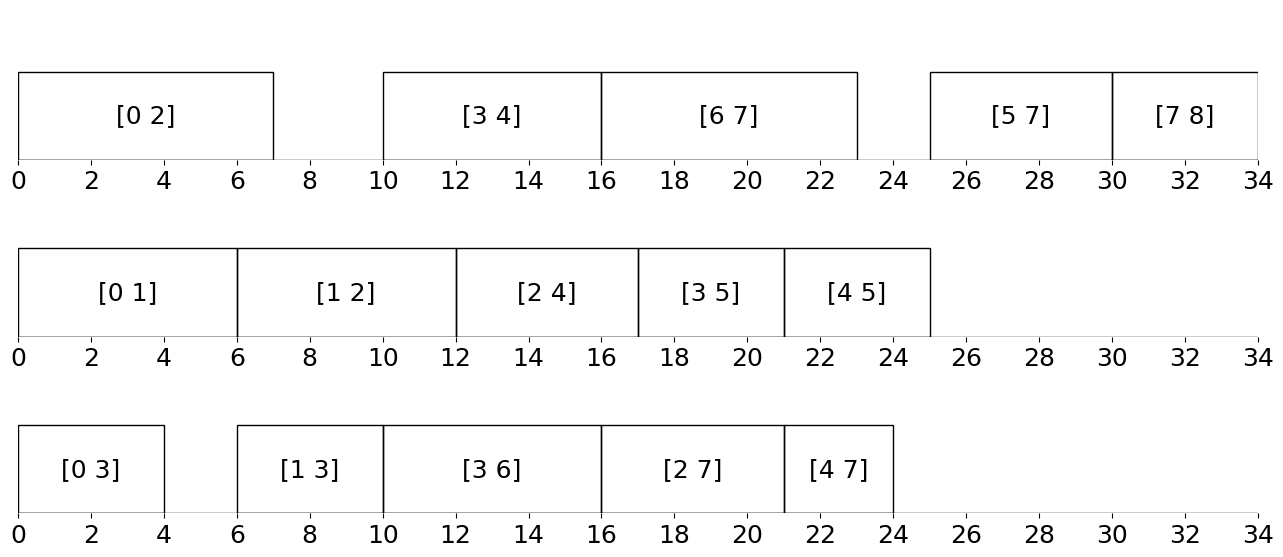
\includegraphics[width=\textwidth]{min-work}
		\caption{Распределение работ по ресурсам (критерий наименьшей длительности работы)}
		\label{fig:min-work}
	\end{center}
\end{figure}

Общее время при данном критерии оказалось равно $T = 34$ часам, при этом первый исполнитель простаивал $3 + 2 = 5$ часов, второй $9$ часов, третий $2 + 10 = 12$ часов.

\newpage

\subsection{Критерий наибольшей длительности работы}

В таблице \ref{tab:max-work} приведено пошаговое решение, полученное с использованием критерия наибольшей длительности работы.

\begin{table}[H]
	\centering
	\def\tabcolsep{5pt}
	\def\arraystretch{1.3}
	\caption{Решение задачи по шагам (критерий наибольшей длительности работы)}
	\label{tab:max-work}
	\begin{tabular}{|c|c|c|c|c|c|c|}
		\hline
		$t$ & $D$ & $E$ & $W$ & $A$ & $B$ & $L$ \\ \hline
		0 & [~] & [0] & [0 1] [0 2] [0 3] & [6 7 4] & [0 3] [0 1] [0 2] & [4 6 7] \\ \hline
		4 & [0 3] & [0] & [~] & [~] & [0 1] [0 2] & [2 3] \\ \hline
		6 & [0 1] & [0 1] & [1 2] [1 3] & [6 4] & [0 2] [1 3] [1 2] & [1 4 6] \\ \hline
		7 & [0 2] & [0 1] & [~] & [~] & [1 3] [1 2] & [3 5] \\ \hline
		10 & [1 3] & [0 1 3] & [3 4] [3 5] [3 6] & [6 4 6] & [1 2] [3 5] [3 4] & [2 4 6] \\ \hline
		12 & [1 2] & [0 1 2 3] & [2 4] [2 7] [3 6] & [5 5 6] & [3 5] [3 4] [2 4] & [2 4 5] \\ \hline
		14 & [3 5] & [0 1 2 3] & [2 7] [3 6] & [5 6] & [3 4] [2 4] [2 7] & [2 3 5] \\ \hline
		16 & [3 4] & [0 1 2 3] & [3 6] & [6] & [2 4] [2 7] [3 6] & [1 3 6] \\ \hline
		17 & [2 4] & [0 1 2 3 4] & [4 5] [4 7] & [4 3] & [2 7] [3 6] [4 7] & [2 5 3] \\ \hline
		19 & [2 7] & [0 1 2 3 4] & [4 5] & [4] & [3 6] [4 7] [4 5] & [3 1 4] \\ \hline
		20 & [4 7] & [0 1 2 3 4] & [~] & [~] & [3 6] [4 5] & [2 3] \\ \hline
		22 & [3 6] & [0 1 2 3 4 6] & [6 7] & [7] & [4 5] [6 7] & [1 7] \\ \hline
		23 & [4 5] & [0 1 2 3 4 5 6] & [5 7] & [5] & [6 7] [5 7] & [6 5] \\ \hline
		28 & [5 7] & [0 1 2 3 4 5 6] & [~] & [~] & [6 7] & [1] \\ \hline
		29 & [6 7] & [0 1 2 3 4 5 6 7] & [7 8] & [4] & [7 8] & [4] \\ \hline
		33 & [7 8] & [0 1 2 3 4 5 6 7 8] & [~] & [~] & [~] & [~] \\ \hline
	\end{tabular}
\end{table}

\newpage

На рис. \ref{fig:max-work} изображено распределение работ по ресурсам, полученное с использованием критерия наибольшей длительности работы.

\begin{figure}[H]
	\begin{center}
		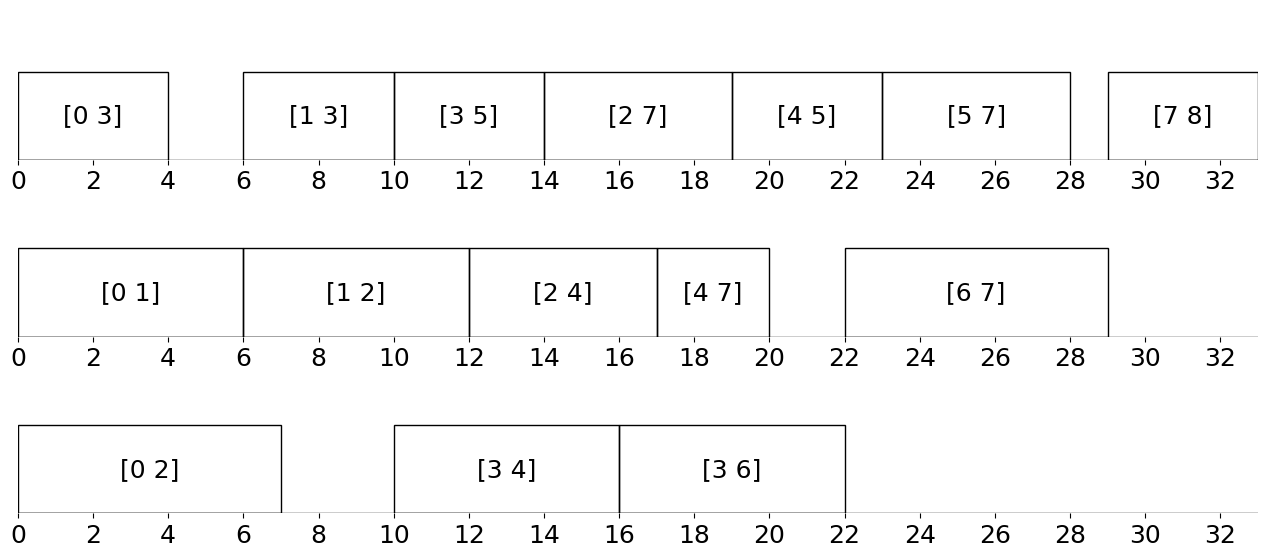
\includegraphics[width=\textwidth]{max-work}
		\caption{Распределение работ по ресурсам (критерий наибольшей длительности работы)}
		\label{fig:max-work}
	\end{center}
\end{figure}

Общее время при данном критерии оказалось равно $T = 33$ часам, при этом первый исполнитель простаивал $2 + 1 = 3$ часа, второй $2 + 4 = 6$ часов, третий $3 + 11 = 14$ часов.

\newpage

\subsection{Критерий наименьшего резерва работы}

В таблице \ref{tab:min-reserve} приведено пошаговое решение, полученное с использованием критерия наименьшего резерва работы.

\begin{table}[H]
	\centering
	\def\tabcolsep{6pt}
	\def\arraystretch{1.3}
	\caption{Решение задачи по шагам (критерий наименьшего резерва работы)}
	\label{tab:min-reserve}
	\begin{tabular}{|c|c|c|c|c|c|c|}
		\hline
		$t$ & $D$ & $E$ & $W$ & $A$ & $B$ & $L$ \\ \hline
		0 & [~] & [0] & [0 1] [0 2] [0 3] & [6 7 4] & [0 3] [0 2] [0 1] & [4 7 6] \\ \hline
		4 & [0 3] & [0] & [~] & [~] & [0 2] [0 1] & [3 2] \\ \hline
		6 & [0 1] & [0 1] & [1 2] [1 3] & [6 4] & [0 2] [1 3] [1 2] & [1 4 6] \\ \hline
		7 & [0 2] & [0 1] & [~] & [~] & [1 3] [1 2] & [3 5] \\ \hline
		10 & [1 3] & [0 1 3] & [3 4] [3 5] [3 6] & [6 4 6] & [1 2] [3 5] [3 6] & [2 4 6] \\ \hline
		12 & [1 2] & [0 1 2 3] & [2 4] [2 7] [3 4] & [5 5 6] & [3 5] [3 6] [2 7] & [2 4 5] \\ \hline
		14 & [3 5] & [0 1 2 3] & [2 4] [3 4] & [5 6] & [3 6] [2 7] [3 4] & [2 3 6] \\ \hline
		16 & [3 6] & [0 1 2 3 6] & [2 4] [6 7] & [5 7] & [2 7] [3 4] [6 7] & [1 4 7] \\ \hline
		17 & [2 7] & [0 1 2 3 6] & [2 4] & [5] & [3 4] [6 7] [2 4] & [3 6 5] \\ \hline
		20 & [3 4] & [0 1 2 3 6] & [~] & [~] & [6 7] [2 4] & [3 2] \\ \hline
		22 & [2 4] & [0 1 2 3 4 6] & [4 5] [4 7] & [4 3] & [6 7] [4 7] [4 5] & [1 3 4] \\ \hline
		23 & [6 7] & [0 1 2 3 4 6] & [~] & [~] & [4 7] [4 5] & [2 3] \\ \hline
		25 & [4 7] & [0 1 2 3 4 6] & [~] & [~] & [4 5] & [1] \\ \hline
		26 & [4 5] & [0 1 2 3 4 5 6] & [5 7] & [5] & [5 7] & [5] \\ \hline
		31 & [5 7] & [0 1 2 3 4 5 6 7] & [7 8] & [4] & [7 8] & [4] \\ \hline
		35 & [7 8] & [0 1 2 3 4 5 6 7 8] & [~] & [~] & [~] & [~] \\ \hline
	\end{tabular}
\end{table}

\newpage

На рис. \ref{fig:min-reserve} изображено распределение работ по ресурсам, полученное с использованием критерия наименьшего резерва работы.

\begin{figure}[H]
	\begin{center}
		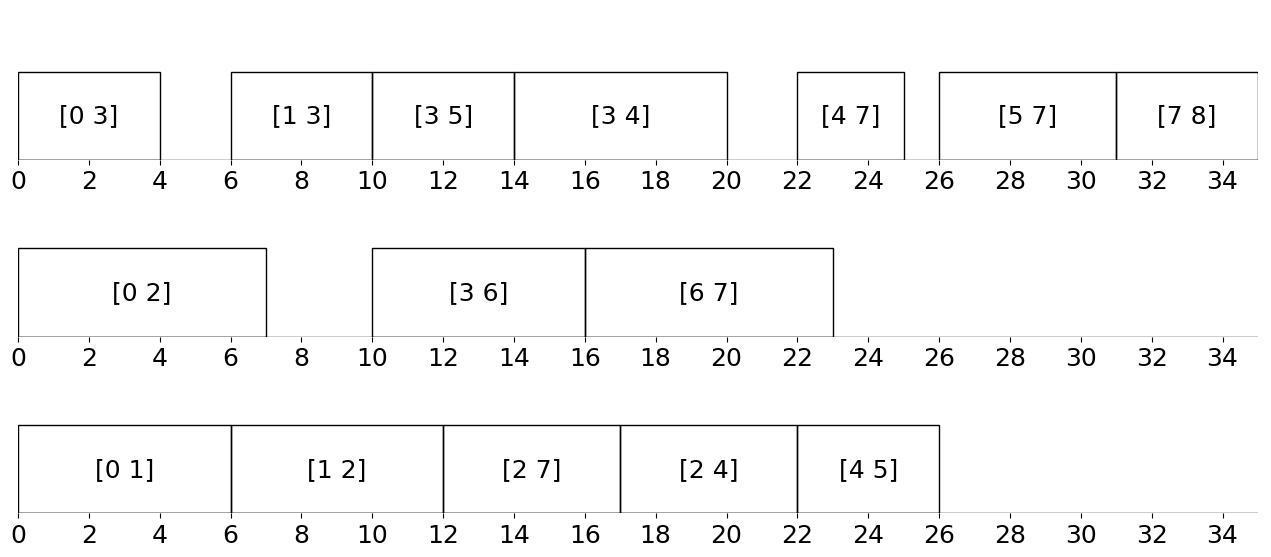
\includegraphics[width=\textwidth]{min-reserve}
		\caption{Распределение работ по ресурсам (критерий наименьшего резерва работы)}
		\label{fig:min-reserve}
	\end{center}
\end{figure}

Общее время при данном критерии оказалось равно $T = 35$ часам, при этом первый исполнитель простаивал $2 + 2 + 1 = 5$ часов, второй $3 + 12 = 15$ часов, третий $9$ часов.

\newpage

\subsection{Критерий наибольшего резерва работы}

В таблице \ref{tab:max-reserve} приведено пошаговое решение, полученное с использованием критерия наибольшего резерва работы.

\begin{table}[H]
	\centering
	\def\tabcolsep{4pt}
	\def\arraystretch{1.3}
	\caption{Решение задачи по шагам (критерий наибольшего резерва работы)}
	\label{tab:max-reserve}
	\begin{tabular}{|c|c|c|c|c|c|c|}
		\hline
		$t$ & $D$ & $E$ & $W$ & $A$ & $B$ & $L$ \\ \hline
		0 & [~] & [0] & [0 1] [0 2] [0 3] & [6 7 4] & [0 1] [0 2] [0 3] & [6 7 4] \\ \hline
		4 & [0 3] & [0] & [~] & [~] & [0 1] [0 2] & [2 3] \\ \hline
		6 & [0 1] & [0 1] & [1 2] [1 3] & [6 4] & [0 2] [1 2] [1 3] & [1 6 4] \\ \hline
		7 & [0 2] & [0 1] & [~] & [~] & [1 2] [1 3] & [5 3] \\ \hline
		10 & [1 3] & [0 1 3] & [3 4] [3 5] [3 6] & [6 4 6] & [1 2] [3 4] [3 6] & [2 6 6] \\ \hline
		12 & [1 2] & [0 1 2 3] & [2 4] [2 7] [3 5] & [5 5 4] & [3 4] [3 6] [2 4] & [4 4 5] \\ \hline
		16 & [3 4] [3 6] & [0 1 2 3 6] & [2 7] [3 5] [6 7] & [5 4 7] & [2 4] [6 7] [3 5] & [1 7 4] \\ \hline
		17 & [2 4] & [0 1 2 3 4 6] & [2 7] [4 5] [4 7] & [5 4 3] & [6 7] [3 5] [4 5] & [6 3 4] \\ \hline
		20 & [3 5] & [0 1 2 3 4 6] & [2 7] [4 7] & [5 3] & [6 7] [4 5] [4 7] & [3 1 3] \\ \hline
		21 & [4 5] & [0 1 2 3 4 5 6] & [2 7] [5 7] & [5 5] & [6 7] [4 7] [5 7] & [2 2 5] \\ \hline
		23 & [6 7] [4 7] & [0 1 2 3 4 5 6] & [2 7] & [5] & [5 7] [2 7] & [3 5] \\ \hline
		26 & [5 7] & [0 1 2 3 4 5 6] & [~] & [~] & [2 7] & [2] \\ \hline
		28 & [2 7] & [0 1 2 3 4 5 6 7] & [7 8] & [4] & [7 8] & [4] \\ \hline
		32 & [7 8] & [0 1 2 3 4 5 6 7 8] & [~] & [~] & [~] & [~] \\ \hline
	\end{tabular}
\end{table}

\newpage

На рис. \ref{fig:max-reserve} изображено распределение работ по ресурсам, полученное с использованием критерия наибольшего резерва работы.

\begin{figure}[H]
	\begin{center}
		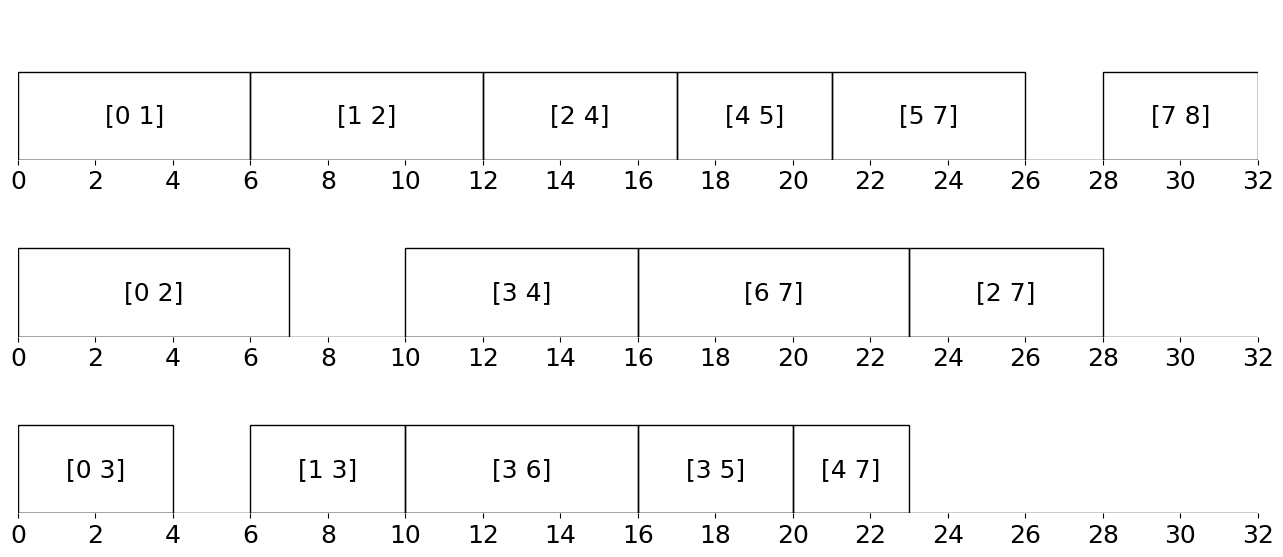
\includegraphics[width=\textwidth]{max-reserve}
		\caption{Распределение работ по ресурсам (критерий наибольшего резерва работы)}
		\label{fig:max-reserve}
	\end{center}
\end{figure}

Общее время при данном критерии оказалось равно $T = 32$ часам, при этом первый исполнитель простаивал $2$ часа, второй $3 + 4 = 7$ часов, третий $2 + 9 = 11$ часов. Таким образом, оптимальными в данном случае оказался критерий наибольшего резерва работы.

\end{document}